\chapter{Umsetzung}
\label{chapter:Umsetzung}

In den folgenden Abschnitten wird auf die Umsetzung der Anwendung sowie des KNN eingegangen.

\section{Umsetzung der Anwendung}
\label{section:Umsetzung der Anwendung}
<<Benedikt>>\Blindtext

\section{Umsetzung des künstlichen neuronalen Netzes mit Neurophstudio} %Sebastian
\label{section:Umsetzung des künstlichen neuronalen Netzes mit Neurophstudio} %Sebastian

In diesem Abschnitt wird beschrieben, wie das KNN aus der Konzeptionsphase (siehe Abbildung 2.3) umgesetzt wurde. Zur Umsetzung wurde die Anwendung `"Neurophstudio"' verwendet. Diese ist ein Teil des Neuroph-Frameworks und erlaubt das Erstellen, Trainieren und Testen von KNN mittels einer graphischen Oberfläche. Das erstellte KNN kann anschließend mittels einer Library in eine Java-Anwendung eingebunden werden.

Nachdem das KNN angelegt wurde, musste dieses noch trainiert und anschließend getestet werden. Für diesen Vorgang sind Trainings- sowie Testdaten nötig. Die benötigten Daten konnten als Excel-Datei von der nachfolgenden Webseite bezogen werden: \textit{http://www.quandl.com/}. Es wurden die letzten $600$ Börsenkurse des DAX extrahiert und anschließend in $2$ Datensätze aufgeteilt: Einen Trainingsdatensatz bestehend aus $450$ Trainingsdaten sowie einen Testdatensatz bestehend aus $150$ Testdaten. Da diese Datensätze noch nicht normalisiert waren, die Daten jedoch in normalisierter Form für das KNN zur Verfügung stehen müssen, wurden diese mit folgender Formel normalisiert:

\begin{equation}\formelentry{Normalisierungsformel}
  N_h = \frac{A-min(A}{max(A)-min(A)}\cdot0,8+01
\end{equation}

Damit wurde sichergestellt, dass sich alle Werte der Datensätze im Intervall $[0,1]$ befinden, wobei die Multiplikation mit $0,8$ sowie die Addition mit $0,1$ Extremwerte abmildern soll.

Nachdem alle Komponenten für die Erstellung eines fertigen KNN vorhanden waren, konnte mit dem Training begonnen werden. Dafür wurden $200.000$ Trainingszyklen gestartet. Als Lernverfahren wurde das Backpropagation-Verfahren mit einer Lernrate von $0,7$ benutzt und als Aktivierungsfunktion eine Sigmoide Funktion. Nachdem das Training abgeschlossen war, wurde das KNN noch noch getestet. Dabei haben sich jeweils die folgenden Werte ergeben:

\begin{table}[H]
\centering
\begin{tabular}{|c|c|}
\hline 
\textbf{Durchlauf} & \textbf{MSE} \\ 
\hline 
Trainingszyklus & 0,001048 \\ 
\hline  
Testzyklus & 0,002134  \\ 
\hline 
\end{tabular} 
\label{tab:ERGGrundnetz}
\caption{Die Trainings- und Testergebnisse des Grundnetzes}
\end{table}

Dieses KNN bildet nun die Grundlage für weitere Optimierungsmaßnahmen.

\section{Optimierung des künstlichen neuronalen Netzes}
\label{section:Optimierung des künstlischen neuronalen Netzes}

Nachdem das Grundmodell des KNN erstellt war, wurde dieses noch weiter optimiert. Darauf wird nun in den Unterabschnitten \ref{subsection:Optimierung der Topologie}, \ref{subsection:Wahl der optimalen Transferfunktion} sowie \ref{subsection:Wahl der optimalen Lernregel} genauer eingegangen. 

\subsection{Optimierung der Topologie}
\label{subsection:Optimierung der Topologie}

Das im Abschnitt \ref{section:Umsetzung des künstlichen neuronalen Netzes mit Neurophstudio} erstellte KNN wird in diesem Abschnitt hinsichtlich der verwendeten Topologie optimiert. Dabei werden sukzessive Neuronen in der Zwischenschicht hinzugefügt bzw. entfernt und für jeden Trainings- und Testverlauf der MSE notiert. Auch wird jede Topologie einmal mit und einmal ohne ein Bias-Neuron trainiert und getestet. die Topologie mit den geringsten MSE im Testverlauf wird dann übernommen. Die Ergebnisse dieser Optimierung können aus der Tabelle \ref{tab:TOPMSE} entnommen werden. Der Term $B$ steht dabei für das Bias-Neuron.

\begin{table}[H]
  \centering
  \begin{tabular}{|c|c|c|c|c|}
  \hline 
  \rule[0ex]{0pt}{2.5ex} Topologie & Training-MSE & Test-MSE & Training-MSE (B) & Test-MSE (B) \\ 
  \hline 
  \rule[0ex]{0pt}{2.5ex} 4-03-1 (B)& 0.000 & 0.000 & 0.000 & 0.000\\ 
  \hline 
  \rule[0ex]{0pt}{2.5ex} 4-05-1 (B)& 0.000 & 0.000 & 0.000 & 0.000\\ 
  \hline 
  \rule[0ex]{0pt}{2.5ex} 4-07-1 (B)& 0.000 & 0.000 & 0.000 & 0.000\\ 
  \hline 
  \rule[0ex]{0pt}{2.5ex} 4-09-1 (B)& 0.000 & 0.000 & 0.000 & 0.000\\ 
  \hline 
  \rule[0ex]{0pt}{2.5ex} 4-11-1 (B)& 0.000 & 0.000 & 0.000 & 0.000\\ 
  \hline 
  \rule[0ex]{0pt}{2.5ex} 4-13-1 (B)& 0.000 & 0.000 & 0.000 & 0.000\\ 
  \hline 
  \end{tabular} 
  \caption{Jeweilige Topologien \& korrespondierende MSE}
  \label{tab:TOPMSE}
\end{table}

Wie aus der Tabelle \ref{tab:TOPMSE} zu erkennen, liefert eine Topologie mit $4$ Input-Neuronen, $7$ versteckten Neuronen, einen Bias-Neuron sowie einen Output-Neuron die besten Werte. Das Start-Topologie aus der ersten Umsetzung wird nun durch diese Topologie ausgetauscht.

\subsection{Wahl der optimalen Transferfunktion} 
\label{subsection:Wahl der optimalen Transferfunktion} 

Nachdem die Topologie des KNN optimiert wurde, wurde noch die Transferfunktion optimiert. Hierbei wurde das Netz einmal mittels einer Sigmoiden Funktion und anschließend nochmals mit einer Tanh-Funktion trainiert und getestet. Dabei ist anzumerken, dass die Tanh-Funktion lediglich ein Sonderfall einer sigmoiden Funktion darstellt (Das wird klarer, wenn man bedenkt, dass "`Sigmoid"' mit "`S-Förmig"' übersetzt werden kann). Die Abbildung \ref{fig:sigtanh}
zeigt nochmals die Bauart der beiden Funktionen auf.

\begin{figure}[H]
\hfill
\subfigure[Sigmoid]{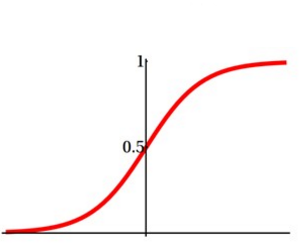
\includegraphics[width=5cm]{Sigmoid.PNG}}
\hfill
\subfigure[Tanh]{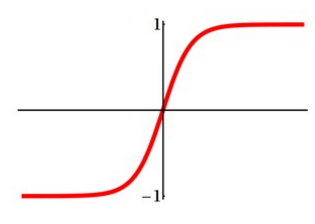
\includegraphics[width=5cm]{tanh.PNG}}
\hfill
\caption{Die Sigmoide Funktion und die Tanh Funktion im Vergleich}
\label{fig:sigtanh}
\end{figure}

\begin{equation}\formelentry{Sigmoide Funktion sowie Tanh Funktion}
(a)\ f(x)= \frac{1}{1+e^{-cx}}\ \ \ \ \ \ \ \ \ \ \ (b)\ f(x)= tanh(x)
\end{equation}


In der Tabelle  \ref{tab:TRANSMSE} können die Ergebnisse dieser Optimierungsschrittes entnommen werden.


\begin{table}[H]
  \centering
  \begin{tabular}{|c|c|}
  \hline 
  \rule[0ex]{0pt}{2.5ex} Transferfunktion & Mean Squared Error \\ 
  \hline 
  \rule[0ex]{0pt}{2.5ex} Sigmoid & 0.000 \\ 
  \hline 
  \rule[0ex]{0pt}{2.5ex} Tanh & 0.000 \\ 
  \hline 
  \end{tabular} 
  \caption{Jeweilige Transferfunktionen \& korrespondierende MSE}
  \label{tab:TRANSMSE}
\end{table}

Man erkennt, dass es bei der bisher genutzten sigmoiden Funktion bereits um die beste Lösung handelt. Folglich wurde das KNN in dieser Hinsicht nicht weiter optimiert und die ursprüngliche Funktion wurde belassen.

\subsection{Wahl der optimalen Lernregel}
\label{subsection:Wahl der optimalen Lernregel}

Als letzten Schritt wurde die Lernregel des KNN optimiert. Innerhalb des Verfahrens der überwachten Lernens existieren mehrere Lernregeln, um das Netz zu trainieren. Die bekannteste Lernregel ist die Backpropagation-Lernregel. Diese Regel gibt es in mehreren Variationen. In dieser Seminararbeit werden zum einen das Grundverfahren sowie einige Variationen, namentlich das  "`Momentum Backpropagation"' sowie das "`Resilient Backpropagation"' beschrieben und untersucht. Anschließend wird das für die Anwendung am besten geeignete Verfahren ausgewählt.

\begin{itemize}
\item \textbf{Backpropagation}:\\
Dies ist das klassische Fehlerrükcführungsverfahren zum Anpassen der Verbindungsgewichte. Die Gewichtsveränderung erfolgt durch einen Fehlersignal, dass aus der Abweichung von tatsächlicher und prognostizierter Ausgabe berechnet wird. Die Gewichtsveränderung erfolgt hierbei schichtweise von den Ausgangsneuronen bis zu den Eingangneuronen.

\item \textbf{Momentum Backpropagation}:\\
Dieses Verfahren fügt dem klassichen Verfahren einen Trägheitsterm hinzu, indem die Gewichtsveränderung zum Zeitpunkt $t-1$ berücksichtigt wird. Der Momentumwert gibt dabei die Sträkre an, wie startk dieser Wert berücksichtigt wird (zwischen 0 und 1).Durch diesen Trägheitsterm wird die Wahrscheinlichkeit, dass das \acs{knn} beim Training in ein lokales Minimum oszilliert und sich somit nicht weiter den Idealwert approximieren kann. Auch die Wahl der Lernrate gestaltet sich hier weniger kritisch. 

\item \textbf{Resilient Backpropagation}:\\
Resilient heißt Federnd. Dieses Verfahren nutzt das Vorzeichen das Gradienten zum Zeitpunkt 

\end{itemize}


Allen drei Lernregeln ist gemein, dass zur Bestimmung des Fehlers zwischen der prognostizierten and tatsächlichen Ausgabe der MSE benutzt werden kann. Die MSE-Formel würde in den konkreten Fall der Anwendung wie folgt lauten:

\begin{equation}\formelentry{MSE zur Berechnung der Abweichung}
   \frac{1}{2}\sum^{n}_{i=1} (KT_{i} - KV_{i})^2
\end{equation}

Wobei $n$ für die Anzahl der Datensätze steht, $KT_i$ für den tatsächlichen Ausgabewert für den Datensatz $i$ steht und $KV_i$ für den prognostizierten Datensatz $i$ steht.





\begin{table}[H]
  \centering
  \begin{tabular}{|c|c|c|}
  \hline 
  \rule[0ex]{0pt}{2.5ex} Lernregel & Mean Squared Error \\ 
  \hline 
  \rule[0ex]{0pt}{2.5ex} Backpropagation & 0.000 \\ 
  \hline 
  \rule[0ex]{0pt}{2.5ex} Momentum Backpropagation & 0.000\\ 
  \hline 
  \rule[0ex]{0pt}{2.5ex} Resilient Propagation & 0.000 \\ 
  \hline 
  \end{tabular} 
  \caption{Jeweilige Lernregeln \& korrespondierende MSE}
  \label{tab:tab3}
\end{table}



\section{Die endgültigen künstlichen neuronalen Netze}
<<Sebastian>> \Blindtext
\section{Zusammenführung der Komponenten}
<<benedikt>> \Blindtext
